\documentclass{report}
\usepackage{fancyhdr} % Required for custom headers
\usepackage{lastpage} % Required to determine the last page for the footer
\usepackage{extramarks} % Required for headers and footers
\usepackage{graphicx} % Required to insert images
%\usepackage{lipsum} % Used for inserting dummy 'Lorem ipsum' text into the template
\usepackage{amsmath}
\usepackage{float}
\usepackage{graphicx} 
%\usepackage{amsfont}
%\usepackage{amssymb}

\usepackage{multicol}
% Margins
\topmargin=-0.5in
\evensidemargin=0in
\oddsidemargin=-0.5in
\textwidth=7.5in
\textheight=9.0in
\headsep=0.25in 


\pagestyle{fancy}

%\rhead{\textbf{Marshall's Recipes}} % Top right header
%\lhead{\textbf{Curry Stir Fry}}
%\chead{ }
%\title{Curry Stir Fry}

\begin{document}
%\vspace{8mm}
%\textbf{PRELIMINARIES:}


\bigskip

\bigskip

\begin{multicols}{2}
\textbf{Ingredients}
\begin{itemize}
\item 1 lb linguine\quad (1620 kCal/ 57 gP/ 8 gF/ 341 gC)
\item 2 lbs peeled \& deveined shrimp \newline(897 kCal/ 218 gP/ 3gF/ 2 gC)
\item 3-4 shallots  \quad (75 kCal/ 3 gP/ 0 gF/ 17 gC)
\item 1 cup dry white wine (I use Pinot Grigio)
\newline  (192 kCal/ 1 gP/ 0gF/ 5 gC)
\item 5 tbsp butter \quad (510 kCal/ 0 gP/ 60 gF/ 0 gC)
\item 5 tbsp. olive oil \quad (510 kCal/ 0 gP/ 60 gF/ 0 gC)
\item $\sim 5$ cloves of garlic (minced) (65 kCal /3 gP/ 0 gF/ 15 gC)
\item The juice of 2 lemons
\item 2 tbsp. red pepper flakes
\item 2 tsp. salt
\item 1 tsp. black pepper
\item $\frac{1}{4}$ cup chopped parsley 



\end{itemize}


\columnbreak
\textbf{Procedure:}
\medskip


\begin{enumerate}
\item Begin by boiling water in a large pot for the pasta. When it has come to boil, add a couple teaspoons of salt and add linguine. Stir to make sure the pasta separates. Cover. When water returns to a boil, cook for 7-9 minutes. Drain pasta. 


\medskip
\item Meanwhile, in a large skillet, melt 2 tbsp of olive oil in 2 tpsb butter over medium-high heat. Saute the shallots, garlic, and red pepper flakes until the shallots are transluscent ($\sim$4 minutes). Season the shrimp with salt and pepper; add them to the pan and cook until they have turned pink. Remove shrimp from pan and keep warm. 
\medskip

\item Add wine and lemon juice and bring to a boil. Add 3 tbsp of olive oil and 3 tbsp of butter. When the butter has melted, return the shrimp to the pan along with parsley and cooked pasta. 
\newline 

 \item Stir well and season with salt and pepper. Drizzle olive oil and serve immediately.   
\end{enumerate}
\begin{table}[H]
  \begin{center}
    \caption{Macro totals}
    \label{tab:table1}
    \begin{tabular}{c|c|c|c} % <-- Alignments: 1st column left, 2nd middle and 3rd right, with vertical lines in between
      \textbf{Calories} & \textbf{Protein} & \textbf{Fat} & \textbf{Carbs}\\
      \hline
      3,869 kCal & 282 g & 134 g & 380 g\\
    \end{tabular}
  \end{center}
\end{table}
\end{multicols}



\begin{center}
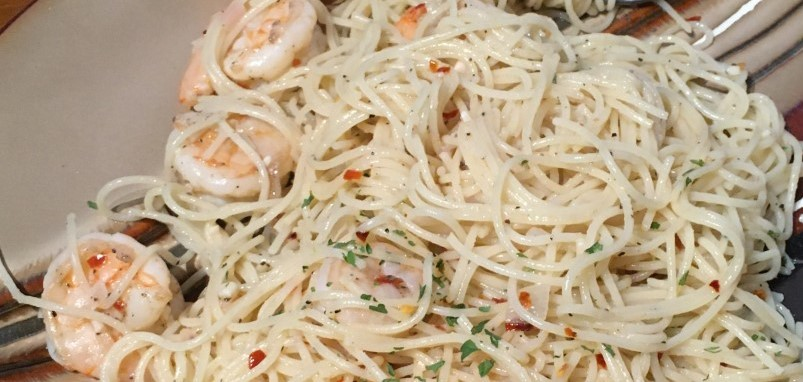
\includegraphics[scale=0.65]{Pasta/Shrimp Scampi/Shrimp Scampi.jpg}
\end{center}


\end{document}